\documentclass{beamer}

\usepackage[utf8]{inputenc}

\usetheme{CambridgeUS}
\usecolortheme{rose}

\useoutertheme{infolines}
\setbeamertemplate{blocks}[default]
\setbeamertemplate{items}[triangle]
\setbeamertemplate{enumerate items}[square]
\setbeamertemplate{sections/subsections in toc}[square]

\newcommand{\mscdiagram}[2][1]{
  \begin{center}
    \includegraphics[height=0.7\paperheight,width=#1\paperwidth,keepaspectratio]{#2}
  \end{center}
}

\newcommand{\fullframepicture}[1]{
  \mode
  {
  }
  \mode{\usebackgroundtemplate{}}
}

\AtBeginSubsection[]
{
  \begin{frame}{Outline}
    \tableofcontents[sectionstyle=show/shaded,subsectionstyle=show/shaded/hide]
  \end{frame}
}

\title{Postgres on the wire}
\subtitle{A look at the PostgreSQL wire protocol}
\author[Jan Urbański]{Jan Urbański \\ \texttt{j.urbanski@wulczer.org}}
\institute{Ducksboard}
\date[PGCon 2014]{PGCon 2014, Ottawa, May 23}

\begin{document}

\frame{\titlepage}

\begin{frame}[fragile]
  \frametitle{For those following at home}

  \begin{block}{Getting the slides}
    \begin{semiverbatim}
    \$ wget http://wulczer.org/postgres-on-the-wire.pdf
    \end{semiverbatim}
  \end{block}

  \begin{block}{Getting the source}
    \begin{semiverbatim}
    \$ https://github.com/wulczer/postgres-on-the-wire
    \end{semiverbatim}
  \end{block}
\end{frame}

\usebackgroundtemplate{
  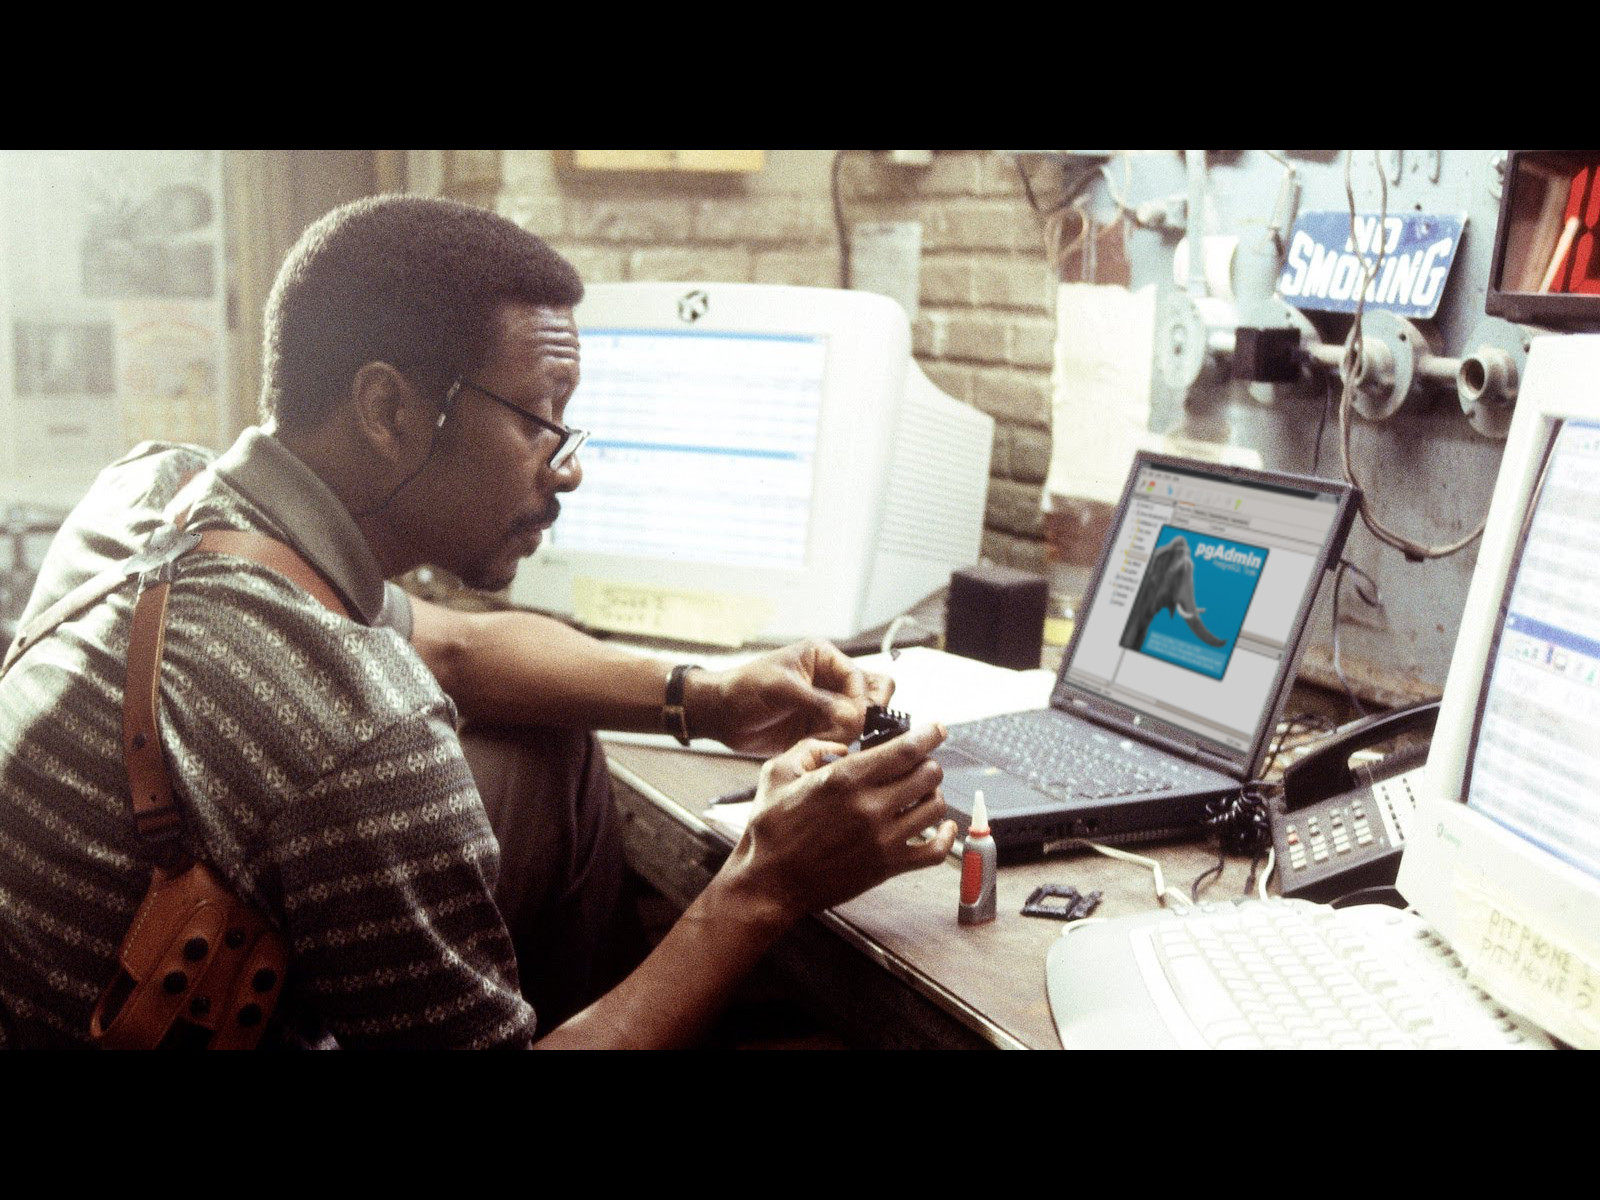
\includegraphics[width=\paperwidth,height=\paperheight]{the-wire.jpg}
}
\begin{frame}[plain]
\end{frame}
\usebackgroundtemplate{}

\begin{frame}
  \tableofcontents
\end{frame}

\section{Protocol basics}
\subsection{Frame format}

\begin{frame}
  \frametitle{Protocol versions}

  \begin{itemize}
  \item the 2.0 protocol got introduced in 6.4, around 1999
    \begin{itemize}
    \item protocol versioning got added in the previous release
    \end{itemize}
  \item the 3.0 got introduced in 7.4, in 2003
  \item the server \alert{still supports} protocol 1.0!
  \item 3.0 has some new features
    \begin{itemize}
    \item extended query protocol
    \item COPY improvements
    \item overall better frame structure
    \end{itemize}
  \end{itemize}
\end{frame}

\begin{frame}
  \frametitle{Handling incoming connections}

  Connections are received by the postmaster process, which immediately forks a
  new process to deal with them.

  \begin{itemize}
  \item any \alert{parsing issues} won't affect the postmaster
  \item authentication is done \alert{after} a process is forked
  \item closing the connection results in \alert{terminating} the backend
    \begin{itemize}
    \item but the backend needs to notice that first
    \item killing the client might not terminate the running query
    \end{itemize}
  \end{itemize}
\end{frame}

\begin{frame}
  \frametitle{FEBE frame format}

  Virtually all messages start with an ASCII identifier, followed by length and
  payload.

  \begin{center}
    \includegraphics[height=1.2cm]{regular-packet}
  \end{center}

  The exception is the startup packet, which starts with the length followed by
  the protocol version.

  \begin{center}
    \includegraphics[height=1.2cm]{startup-packet}
  \end{center}

\end{frame}

\begin{frame}
  \frametitle{Startup packet}

  \begin{center}
    \includegraphics[height=1cm]{startup-packet-detail}
  \end{center}

  \begin{itemize}
  \item the very first bit of data received by the backend is parsed as the
    startup packet
  \item starts with a 32 bit \alert{protocol version} field
  \item in protocol 2.0 it had a fixed length, in 3.0 it's variable length
  \item what follows is a list of key/value pairs denoting options
    \begin{itemize}
    \item some keys, like \texttt{user}, \texttt{database} or \texttt{options} are special
    \item the rest are generic GUC options
    \end{itemize}
  \end{itemize}
\end{frame}

\begin{frame}
  \frametitle{Regular data packet}

  \begin{center}
    \includegraphics[height=1cm]{regular-packet}
  \end{center}

  \begin{itemize}
  \item starts with an ASCII \alert{identifier}
  \item a 32 bit message length follows
    \begin{itemize}
    \item this means you can't send a query that's larger than 1 GB
    \end{itemize}
  \item interpretation of the payload depends on the identifier
  \end{itemize}
\end{frame}

\subsection{Message flow}

\begin{frame}
  \frametitle{Authentication}

  \begin{center}
    \includegraphics[height=1cm]{authentication-request}
  \end{center}

  \begin{itemize}
  \item if a connection requires authentication, the backend will send a
    AuthenticationRequest
  \item there are several authentication types that can be demanded
    \begin{itemize}
    \item plain-text or MD5 password
    \item it's \alert{up to the server} to require plain text or encrypted
    \item GSSAPI, SSPI
    \end{itemize}
  \item if no auth is necessary, the server sends AuthenticationOK
  \end{itemize}
\end{frame}

\begin{frame}
  \frametitle{Encrypted password exchange}

  \begin{center}
    \includegraphics[height=1cm]{authentication-request-md5}
  \end{center}

  The MD5 AuthenticationRequest message includes a 4 byte salt.

  \begin{align*}
    pwdhash\;&=\;md5(password\;+\;username).hexdigest() \\
    hash\;&=\;'md5'\;+\;md5(pwdhash\;+\;salt).hexdigest()
  \end{align*}

  \begin{itemize}
  \item using a salt prevents \alert{replay attacks}
  \item double-hashing allows the server to only store \alert{hashes}
  \end{itemize}
\end{frame}

\begin{frame}
  \frametitle{Parameter status}

  \begin{center}
    \includegraphics[height=1cm]{parameter-status}
  \end{center}

  \begin{itemize}
  \item the server notifies clients about important parameters
  \item first batch of ParameterStatus messages is sent on startup
    \begin{itemize}
    \item some of them are \alert{informative}, like \texttt{server\_version}
    \item others are critical for \alert{security}, like \texttt{client\_encoding}
    \item others yet are important for the \alert{client}, like \texttt{DateStyle}
    \end{itemize}
  \item when any of those parameters gets set, the server notifies the client
    on the next occasion
  \end{itemize}
\end{frame}

\begin{frame}
  \frametitle{Basic message flow}

  \mscdiagram{basic-message-flow}
\end{frame}

\begin{frame}
  \frametitle{Encryption}

  \begin{center}
    \includegraphics[height=1cm]{ssl-negotiation}
  \end{center}

  \begin{itemize}
  \item the startup packet can use a \alert{dummy protocol version} to ask for
    SSL support
  \item the server responds with with \alert{status byte} or an error message
  \item the client can reconnect or abort if the response is negative
  \end{itemize}
\end{frame}

\begin{frame}
  \frametitle{SSL message flow}

  \mscdiagram{ssl-message-flow}
\end{frame}

\begin{frame}
  \frametitle{Cancellation}

  \begin{center}
    \includegraphics[height=1cm]{cancel-request}
  \end{center}

  \begin{itemize}
  \item the \alert{cancel key} is transmitted by the server upon connection
  \item cancelling queries requires opening \alert{separate connection}
  \item another dummy protocol version is sent to ask for cancellation
  \item the cancellation message includes the process ID and a 32 bit key
    \begin{itemize}
    \item theoretically open to \alert{replay attacks}, but can be sent over
      SSL
    \item libpq \alert{does not}, so most applications will transmit it in the
      open
    \end{itemize}
  \end{itemize}
\end{frame}

\begin{frame}
  \frametitle{Handling errors}

  \begin{center}
    \includegraphics[height=1cm]{error-response}
  \end{center}

  \begin{itemize}
  \item the ErrorResponse message is sent for all kinds of errors
    \begin{itemize}
    \item both for authentication errors and client errors
    \end{itemize}
  \item it is a list of key-value fields
    \begin{itemize}
    \item in 2.0 it was just a string, in 3.0 it has structure
    \item example error fields are: message, detail, hint and error position
    \item detailed down to the source file and line, great for fingerprinting
    \end{itemize}
  \end{itemize}
\end{frame}

\begin{frame}
  \frametitle{Tools}

  \begin{itemize}
    \item standard tools like tcpdump or tshark work
    \item Wireshark has built-in support for deparsing the protocol
      \begin{itemize}
      \item but only for protocol 3.0
      \end{itemize}
    \item pgShark is a very nice tool that works with the Postgres protocol
  \end{itemize}
\end{frame}

\begin{frame}[fragile]
  \frametitle{pgShark examples}

  \begin{block}{generate a report from a pcap file}
    \begin{semiverbatim}
    \$ pgs-badger < dump.pcap
    \end{semiverbatim}
  \end{block}

  \begin{block}{display live protocol info}
    \begin{semiverbatim}
    \$ pgs-debug --interface eth0
    \end{semiverbatim}
  \end{block}

  \begin{block}{dump SQL from a 2.0 protocol connection on a nonstandard port}
    \begin{semiverbatim}
    \$ pgs-sql -2 --port 5433
    \end{semiverbatim}
  \end{block}
\end{frame}

\section{Sending queries}
\subsection{Simple protocol}

\begin{frame}
  \frametitle{Binary vs text data}

  \begin{itemize}
  \item every type has a text and binary representation
  \item depending on \alert{compile-time options}, timestamps are either 64 bit
    integers or floating point values
    \begin{itemize}
    \item this is why \texttt{integer\_datetimes} is sent in ParameterStatus
    \end{itemize}
  \item the client can choose if they want text or binary data
  \item the exact format for each type doesn't seem to be documented anywhere
    \begin{itemize}
    \item but that's what C code is for :)
    \end{itemize}
  \end{itemize}
\end{frame}

\begin{frame}
  \frametitle{Simple query protocol}

  \begin{itemize}
  \item client sends an SQL command
  \item server replies with RowDescription detailing the structure
    \begin{itemize}
    \item each column has a name
    \item the type OID, length and modifier (like \texttt{char(16)})
    \item each column is marked as containing binary or text output
    \end{itemize}
  \item after that a DataRow message is sent for every row
  \item finally, the server sends CommandComplete and ReadyForQuery
  \end{itemize}
\end{frame}

\begin{frame}
  \frametitle{Simple query frames}

  \begin{center}
    \includegraphics[height=1cm]{query}
  \end{center}

  \bigskip

  \hspace{0.4cm}\includegraphics[height=0.9cm]{row-description-top}\;\raisebox{0.2cm}{$+$} \\
  \hspace{0.4cm}\includegraphics[height=0.6cm]{row-description-bottom} \\
  \hspace{0.4cm}\dots

  \bigskip

  \begin{center}
    \includegraphics[height=1cm]{data-row}
  \end{center}

\end{frame}

\begin{frame}
  \frametitle{Simple query frames cont.}

  \begin{center}
    \includegraphics[height=1cm]{command-complete}
  \end{center}

  \bigskip

  \begin{center}
    \includegraphics[height=1cm]{ready-for-query}
  \end{center}

\end{frame}

\begin{frame}[fragile]
  \frametitle{Detecting transaction status}

  \begin{itemize}
  \item the ReadyForQuery message includes \alert{transaction status}
  \item this is useful for things like psql's prompt or, more importantly,
    pgbouncer
  \item the transaction status only got included in protocol 3.0
    \begin{itemize}
    \item for 2.0 libpq does string comparison to try and track the status
    \end{itemize}
  \end{itemize}

  \begin{block}<2->{fe-protocol2.c}
    \begin{semiverbatim}
    By watching for messages (...), we can do a passable
    job of tracking the xact status.  BUT: this does not
    work at all on 7.3 servers with AUTOCOMMIT OFF.
    (Man, was that feature ever a mistake.)  Caveat user.
    \end{semiverbatim}
  \end{block}
\end{frame}

\begin{frame}
  \frametitle{Simple query protocol cont.}

  \begin{itemize}
  \item \alert{several commands} can be sent in one query string
    \begin{itemize}
    \item the server sends one CommandComplete per query
    \item in case of errors it's up to the client to figure out which one failed
    \end{itemize}
  \item sending an empty string yields a special EmptyQueryResponse instead of
    CommandComplete
  \item the simple protocol \alert{always} returns text data, except for binary cursors
  \end{itemize}
\end{frame}

\begin{frame}
  \frametitle{Simple query protocol flow}

  \mscdiagram{simple-query-protocol}
\end{frame}

\subsection{Extended protocol}
\begin{frame}
  \frametitle{Extended query protocol}
  \setbeamercolor{sqlinjection}{bg=block title.bg}

  \begin{itemize}
  \item query execution is split into \alert{separate steps}
  \item each step is confirmed by a separately server message, but they can be
    sent \alert{consecutively} without waiting
  \item allows separating parameters from the query body
  \end{itemize}
  \begin{beamercolorbox}[center,sep=1em]{sqlinjection}
    \only<1>{
      \texttt{SELECT admin FROM users WHERE login = '\alert{\$var}'}
    }
    \only<2-3>{
      \texttt{SELECT admin FROM users WHERE login = '\alert{x' or 1=1; --}'}
    }
    \only<4->{
      \texttt{SELECT admin FROM users WHERE login = \alert{\$1}}
    }
  \end{beamercolorbox}

  \begin{itemize}
  \item disallows sending several commands in one query
  \end{itemize}

  \begin{beamercolorbox}[center,sep=1em]{sqlinjection}
    \only<1-2>{
      \texttt{SELECT * FROM posts WHERE id = \alert{\$var}}
    }
    \only<3>{
      \texttt{SELECT * FROM posts WHERE id = \alert{1; delete from posts;}}
    }
    \only<4->{
      \texttt{SELECT * FROM posts WHERE id = \alert{\$1}}
    }
  \end{beamercolorbox}
\end{frame}

\begin{frame}
  \frametitle{Parse messages}

  \begin{center}
    \includegraphics[height=1cm]{parse}
  \end{center}

  \begin{itemize}
  \item first, the client sends a Parse message with the query string
  \item it can contain \alert{placeholders} (\texttt{\$1, \$2, ...}) for
    parameters
  \item for each parameter you can specify its \alert{type}
    \begin{itemize}
    \item disambiguate between \texttt{select foo(1)} and \texttt{select foo('x')}
    \end{itemize}
  \item the statement can be optionally given a \alert{name}
    \begin{itemize}
    \item unnamed statements live until the next unnamed statement is parsed
    \item named statements need to be explicitly deallocated
    \end{itemize}
  \end{itemize}
\end{frame}

\begin{frame}
  \frametitle{Bind messages}

  \hspace{2cm}\includegraphics[height=0.9cm]{bind-1}\;\raisebox{0.2cm}{$+$} \\
  \hspace{2cm}\includegraphics[height=0.6cm]{bind-2}\;\raisebox{0.2cm}{$+$} \\
  \hspace{2cm}\includegraphics[height=0.6cm]{bind-3}\;\raisebox{0.2cm}{$+$} \\
  \hspace{2cm}\includegraphics[height=0.6cm]{bind-4}

  \begin{itemize}
  \item after the query is parsed, the clients \alert{binds} its parameters
  \item an \alert{output portal} is created for a previously parsed statement
    \begin{itemize}
    \item an empty string can be used for the portal name
    \end{itemize}
  \item for each parameter, its \alert{format} (binary or text) and \alert{value} are specified
  \item finally, for each output column, the requested \alert{output format} is
    sent
  \end{itemize}
\end{frame}

\begin{frame}
  \frametitle{Interlude - Describe messages}


  \begin{center}
    \includegraphics[height=1cm]{describe} \\

    \bigskip

    \includegraphics[height=1cm]{parameter-description}
  \end{center}

  \begin{itemize}
  \item clients can ask for a description of a statement or a portal
  \item \alert{statement} descriptions are returned as two separate messages:
    ParameterDescription and RowDescription
  \item \alert{portal} descriptions are just RowDescriptions
  \item clients can use Describe to make sure they know how to handle data
    being returned
  \end{itemize}
\end{frame}

\begin{frame}
  \frametitle{Execute messages}

  \begin{center}
    \includegraphics[height=1cm]{execute}
  \end{center}

  \begin{itemize}
  \item once the output portal is created, it can be \alert{executed}
  \item the output portal is referred to by name
  \item can specify the \alert{number of rows} to return, or 0 for all rows
  \item a series of DataRow messages follow
  \item no RowDescription is sent
  \end{itemize}
\end{frame}

\begin{frame}
  \frametitle{Execute messages cont.}

  \begin{itemize}
  \item after the portal has been \alert{run to completion}, CommandComplete is
    sent
  \item if the requested number of rows is \alert{less} than what the portal would
    return a PortalSuspended message is sent
  \item AFAIK, only JDBC actually exposes limits for Execute
  \item libpq doesn't even have code to handle PortalSuspended...
  \end{itemize}
\end{frame}

\begin{frame}
  \frametitle{Sync messages}

  \begin{center}
    \includegraphics[height=1cm]{sync}
  \end{center}

  \begin{itemize}
  \item an extended protocol query should end with a Sync
  \item upon receiving Sync the server \alert{closes the transaction} if it was
    implicit and responds with a ReadyForQuery message
  \item in case of earlier errors, the server sends an ErrorResponse and then
    skips until it sees a Sync
  \end{itemize}
\end{frame}

\begin{frame}
  \frametitle{Extended query protocol summary}

  \begin{itemize}
  \item queries are \alert{parsed} at Parse stage
  \item queries are \alert{planned} at Bind stage
  \item queries are \alert{executed} at Execute stage
  \item with statement logging, these three steps will be \alert{timed} and
    \alert{logged separately}
  \end{itemize}
\end{frame}

\begin{frame}
  \frametitle{Extended query protocol flow}

  \begin{columns}[onlytextwidth]
    \begin{column}{0.5\textwidth}
      \mscdiagram[0.4]{extended-query-protocol-1}
    \end{column}
    \begin{column}{0.5\textwidth}
      \mscdiagram[0.4]{extended-query-protocol-2}
    \end{column}
  \end{columns}
\end{frame}

\begin{frame}
  \frametitle{Advanced extended protocol usage}

  \begin{columns}[onlytextwidth]
    \begin{column}{0.5\textwidth}
      \mscdiagram[0.4]{extended-query-protocol-adv-1}
    \end{column}
    \begin{column}{0.5\textwidth}
      \mscdiagram[0.4]{extended-query-protocol-adv-2}
    \end{column}
  \end{columns}
\end{frame}

\section{Other features}
\subsection{The COPY subprotocol}

\begin{frame}
  \frametitle{Entering COPY mode}

  \begin{center}
    \includegraphics[height=1cm]{copy-in}
  \end{center}

  \begin{itemize}
  \item sending \texttt{COPY FROM STDIN} or \texttt{COPY TO STDIN} puts the
    connection in COPY mode
  \item this can happen both during simple and extended query processing
  \item CopyInResponse and CopyOutResponse indicate that the backend has
    switched to COPY mode
  \item they specify the overall format (text or binary) and the format for
    each column
    \begin{itemize}
    \item currently if the overall format is binary, all columns are binary
    \end{itemize}
  \end{itemize}
\end{frame}

\begin{frame}
  \frametitle{Sending COPY data}

  \begin{center}
    \includegraphics[height=1cm]{copy-data}
  \end{center}

  \begin{itemize}
  \item CopyData messages are simply \alert{binary blobs}
  \item to stop \texttt{COPY FROM}, the client can send a CopyFail message
  \item when transfer is complete, the client sends CopyDone
  \item in case of backend errors, an ErrorResponse is sent
  \item there is no way for the frontend to stop a \texttt{COPY TO} operation,
    short of cancelling or disconnecting
  \end{itemize}
\end{frame}

\begin{frame}
  \frametitle{COPY subprotocol flow}

  \mscdiagram{copy-flow}
\end{frame}

\subsection{Less known FEBE features}
\begin{frame}
  \frametitle{Asynchronous operation}

  \begin{center}
    \includegraphics[height=1cm]{notification-response}
  \end{center}

  \begin{itemize}
  \item some messages can appear at \alert{any moment} during the connection
    \begin{itemize}
    \item ParameterStatus
    \item NoticeResponse
    \item NotificationResponse
    \end{itemize}
  \item NOTIFY messages are only sent when a transaction is committed, but you
    should expect them at any time
  \item notices can be sent at any moment
  \end{itemize}
\end{frame}

\begin{frame}
  \frametitle{Fast-path interface}

  \hspace{1cm}\includegraphics[height=0.9cm]{function-call-1}\;\raisebox{0.2cm}{$+$} \\
  \hspace{1cm}\includegraphics[height=0.6cm]{function-call-2}\;\raisebox{0.2cm}{$+$} \\
  \hspace{1cm}\includegraphics[height=0.6cm]{function-call-3}

  \begin{itemize}
  \item a specialised interface for \alert{calling functions}
  \item separate protocol message, FunctionCall, similar to Query
    \begin{itemize}
    \item the function is identified by its OID
    \item arguments format and values are specified similar to Bind
    \end{itemize}
  \item libpq documentation calls it ``\alert{somewhat obsolete}'' :)
  \item can be substituted by a named Parse followed by Bind/Execute
  \item still used by libpq for large object functions
  \end{itemize}
\end{frame}

\begin{frame}
  \frametitle{Replication subprotocol}

  \begin{itemize}
  \item entered using a special \texttt{replication} parameter in the startup
    packet
  \item switches the server to a mode where only the simple query protocol can
    be used
  \item instead of SQL, the server accepts replication commands
    \begin{itemize}
    \item for example, \texttt{START\_REPLICATION} or \texttt{BASE\_BACKUP}
    \end{itemize}
  \item responses are a mix of RowDescription/DataRow and COPY subprotocol data
  \end{itemize}
\end{frame}

\subsection{Future development}
\begin{frame}
  \frametitle{Protocol version 4.0}

  There are \alert{surprisingly few} gripes about protocol 3.0, but some
  proposals have been floated on the development list.

  \begin{itemize}
  \item protocol compression
  \item adding nullable indicator to RowDescription
  \item multi-stage authentication, allowing falling back to a different
    authentication method
  \item negotiating the protocol version
  \item in-band query cancellation
  \item sending per-statement GUC
  \end{itemize}
\end{frame}

\subsection*{Questions}

\begin{frame}
\begin{beamercolorbox}[center]{note}
  \Huge Questions?
\end{beamercolorbox}
\end{frame}

\end{document}
